% !TEX TS-program = pdfLaTeX+shellescape
% !TEX encoding = UTF-8 Unicode

\documentclass{standalone}
\usepackage{pgfplots}
\pgfplotsset{compat=1.18}
\usepgfplotslibrary{fillbetween}

\begin{document}
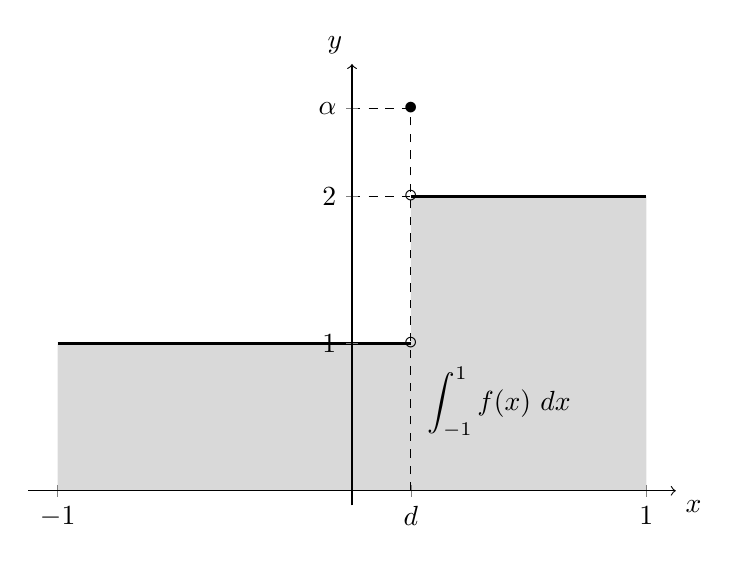
\begin{tikzpicture}
\begin{axis}[
axis on top,
axis lines = middle,
unit vector ratio=2 1, 
% axis equal=false,
scale=1.2, 
xmin=-1.1, xmax=1.1, ymin=-0.1, ymax=2.90, 
% grid = major,
xtick={-1, 0, 0.2, 1},
ytick={0, 1, 2, 2.6},
xticklabels = {$-1$,,$d$, $1$},
yticklabels = {, $1$, $2$, $\alpha$},
xlabel=$x$,
ylabel=$y$,
xlabel style={below right},
ylabel style={above left},
axis line style = {->},
]

\pgfmathsetmacro{\d}{0.2} 
\pgfmathsetmacro{\valpha}{2.6}

% \fill[gray!30] (axis cs: -1, 0) rectangle (axis cs: \d, 1);
\addplot[domain=-1:\d, name path=axis] {0}; 
\addplot[thick, domain=-1:\d, name path=line] {1}; 
\addplot[fill=gray!30] fill between [of=axis and line]; 
\addplot[domain=\d:1, name path=axis] {0}; 
\addplot[thick, domain=\d:1, name path=line] {2}; 
\addplot[fill=gray!30] fill between [of=axis and line]; 
\addplot[thick, domain=\d:1] {2}; 
\node at (axis cs: \d, 1.0) {$\circ$}; 
\node at (axis cs: \d, \valpha) {$\bullet$}; 
\node at (axis cs: \d, 2.0) {$\circ$}; 
\addplot[dashed, domain=0:\d] {2}; 
\addplot[dashed, domain=0:\d] {\valpha}; 
\addplot[dashed, domain=0:\valpha] ({\d}, {\x});
\node at (axis cs: 0.5, 0.6) {$\displaystyle\int_{-1}^1 f(x)~dx$};


% \pgfplotsforeachungrouped \i in {0,...,\Nsub-1}{
%     \pgfmathsetmacro{\xleft}{\a+\i*\h}
%     \pgfmathsetmacro{\xright}{\a+(\i+1)*\h} 
%     \pgfmathsetmacro{\xmid}{\a+(\i+0.5)*\h}
%     \pgfmathsetmacro{\height}{myfunc(\xmid,\a)} 
%     \edef\doplot{\noexpand 
%         \fill[gray!30] (axis cs:{\xleft},{0}) rectangle (axis cs:{\xright},{\height}); 
%     }
%     \doplot
%     \edef\doplot{\noexpand 
%         \draw (axis cs:{\xleft},{0}) rectangle (axis cs:{\xright},{\height});
%     }
%     \doplot
% }

% \addplot [style=thick, domain=0.2:1.2, samples=100] {(sin(deg(2*pi*(x-0.2)))+0.6)/6};

\end{axis}
\end{tikzpicture}


\end{document}